\documentclass{article}
\usepackage{arxiv}
\usepackage{cite}
\usepackage{amsmath, amsfonts, bm, hyperref, siunitx, algorithm, algpseudocode}

\usepackage{tikz}
\usetikzlibrary{shapes.geometric, arrows.meta}
\tikzstyle{process} = [
    rectangle, minimum width=2cm, minimum height=1.3cm, text centered, 
    draw=black
]
\tikzstyle{arrow} = [thick,->,>={Stealth[scale=1.1]}]

\usepackage{graphicx}
\graphicspath{ {../data/} }

\hypersetup{
	pdfauthor={Yuanhao JIANG},
	pdftitle={
        Mathematics of Reinforcement Learning with Applications to 
        Quantitative Finance
    },
	pdfkeywords={
        Reinforcement Learning,  Artificial Neural Networks, Quantitative 
        Finance
    },
	pdfsubject={
        Describe Mathematics of Reinforcement Learning with Applications to 
        Quantitative Finance
    },
}

\begin{document}
\title{
    Mathematics of Reinforcement Learning with Applications to Quantitative 
    Finance
}
\author{
    Yuanhao JIANG\thanks{
        Current student at the University of Edinburgh.
    } \\
	School of Mathematics\\
	The University of Edinburgh\\
	Edinburgh, UK \\
	\texttt{s2132254@ed.ac.uk} \\
}

\maketitle

\begin{abstract}
\noindent This paper provides a new way of pricing in the car insurance
industry, which is, using reinforcement learning algorithms to train pricing 
agents to promote proper price, such that our customer is most likely to 
purchase our product, and we also get the highest profit and a better 
portfolio. 
We first introduce general reinforcement learning knowledge, including how 
we model the interaction between agent and environment using Markov decision
process, and the mathematics behind those methods to solve the reinforcement 
learning problem, especially the Actor-Critic algorithm.
Then we start building the environment, and use artificial neural networks as 
our pricing models, and writing algorithms that are specific to our financial 
problem. 
In the end, we will compare the Actor-Critic algorithms with other popular 
algorithms including REINFORCE and PPO in terms of their rate of convergence 
to a stable reward.
\end{abstract}

\keywords{
    Reinforcement Learning \and 
    Artificial Neural Networks \and 
    Quantitative Finance
}

\tableofcontents

\section{Introduction}
\noindent Modern way of calculating car insurance premium is by estimating
how much risk the customer poses to the insurance provider, and more risk 
results in higher premium. 
The estimation of the risk for a customer is usually done by comparing various
risk factors with the statistics of the database collected so far. Those 
factors might include customer's age, address, occupation, car's mileage, 
brand and model, and so on. For example, younger drivers pose higher risks 
since they are more likely to have an accident due to the lack of driving 
experience compare to elder drivers.
\vspace{2mm}\newline In this paper, instead of using the above method to 
promote car insurance, we use RL methods to train agents that will interact 
with the market and response with price. More specifically, we consider the 
insurance promoting scenario as markov decision process, with the current 
state being the current customer features and current portfolio. At each time
step, the agent promote a price according to the current customer features and
the current portfolio, after that the customer resopnse to the promotion. The 
reward is then given besed on the customer response and the portfolio. Then 
the portfolio updates and a new customer arrives. This set up will help us to
solve the poblem in the context of reinforcement learning, further details are
discussed in the remaining sections.

\section{Reinforcement Learning}
\noindent The reinforcement learning method we want to use is based on the Markov 
decision process (MDP)~\cite{Sutton1998, menache2005basis}, as illustrated in 
Figure~\ref{fig:MDP-illustration}.
\begin{figure}[H]
    \centering
    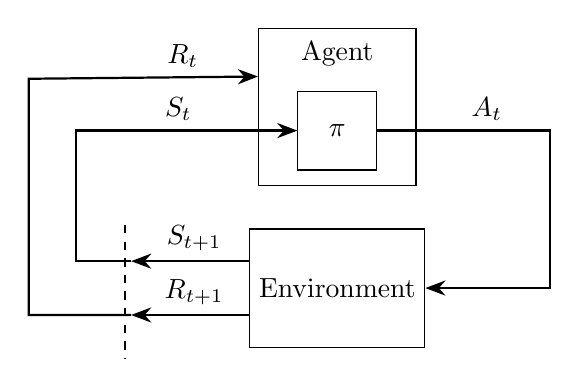
\begin{tikzpicture}
        \node (agent) [process, minimum width=2cm, minimum height=2cm,
            label={[anchor=north,inner sep=5pt]north:Agent}]{};
        \node (pi) [process, left of=agent, minimum width=1cm, 
            minimum height=1cm,xshift=1cm, yshift=-0.3cm] {\(\pi\)};
        \node (env) [process, minimum height=1.5cm, below of=pi, yshift=-1cm] 
            {Environment};

        \draw [arrow] (env.163) -- ++(-1.5,0) node[anchor=south, xshift=0.8cm]
            {\(S_{t+1}\)} coordinate(a1);
        \draw [arrow] (a1) -- ++(-0.7,0) |- node[anchor=south, xshift=1.3cm] 
            {\(S_t\)} (pi);
        \draw [arrow] (env.197) -- ++(-1.5,0) node[anchor=south, xshift=0.8cm]
            {\(R_{t+1}\)} coordinate(a2);
        \draw [arrow] (a2) -- ++(-1.3,0) -- ++(0,3) 
            -- node[anchor=south, xshift=0.5cm] {\(R_t\)} (agent.159);
        \draw [arrow] (pi) -- ++(2.7,0) node[anchor=south, xshift=-0.8cm] 
            {\(A_t\)} |- (env);
        \draw [dashed,thick] (-2.7,-1.5) -- (-2.7, -3.2);
    \end{tikzpicture}
    \caption{MDP Illustration~\cite{Sutton1998}}
    \label{fig:MDP-illustration}
\end{figure}
\noindent However, in RL, the agent is not told which actions to take, but 
instead must discover which actions yield the most reward by trying them. Our 
goal at each time step is to find a policy \(\pi\) to maximize the expected 
reward alonge the process afterwards, which is given by the value function
\[V(s)=\mathbb{E}\left[\sum_{i=0}^{\infty} \gamma^i R_{t+i+1}\;\middle|\; 
S_t=s\right]\]
To achieve this, we need to evaluate the current policy, and improve it 
accordingly.

\subsection{Policy Evaluation}
\noindent We want to evaluate the value function under a given policy \(\pi\).
According to Bellman equation,
\[v_\pi(s)=\mathbb{E}_\pi\left[R_{t+1}+\gamma v_\pi(S_{t+1})\;\middle|\;
S_t=s\right]\]
We can use it to iteratively compute \(v_\pi\). The iteratively update is
\[v_{k+1}(s)=\mathbb{E}_\pi\left[R_{t+1}+\gamma v_k(S_{t+1})\;\middle|\;
S_t=s\right]\]
which is proven that it will converge to the true value given any initial value 
function.

\subsection{Policy Improvement}
\noindent Now we have the evaluated value function for the policy, we want to 
improve it accordingly. To do this, we introduce the q-function under 
policy \(\pi\)~\cite{Sutton1998}
\[q_\pi(s, a) = \mathbb{E}\left[R_{t+1} + \gamma v_\pi(S_{t+1})\;\middle|\;
S_t=s, A_t=a\right]\]
The policy improvement theorem says that, let \(\pi\) and \(\pi'\) be any pair
of policy, for all \(s\) we have
\[q_\pi(s, \pi'(s))\geq v_\pi(s) \:\Rightarrow\: v_{\pi'}(s) \geq v_\pi(s)\]
Now we can improve the policy by
\[\pi'(s)=\underset{a}{\text{argmax}}\:q_\pi(s,a)\]
for all \(s\).

\subsection{Policy Iteration}
\noindent By iteratively applying policy evaluation and policy improvement, we
can obtain a sequence of monotonically improving policies and value 
functions~\cite{Sutton1998} :
\[\pi_0 \overset{E}{\longrightarrow} v_{\pi_0} \overset{I}{\longrightarrow}
\pi_1 \overset{E}{\longrightarrow} v_{\pi_1} \overset{I}{\longrightarrow}
\dots \overset{I}{\longrightarrow} \pi_* \overset{E}{\longrightarrow} v_*\]
where \(\overset{E}{\longrightarrow}\) denotes a policy evaluation and
\(\overset{I}{\longrightarrow}\) denotes a policy improvement. This way of 
finding an optimal policy is called policy iteration.

\subsection{Value Iteration}
\noindent One drawback to policy iteration is that each of its iterations 
involves policy evaluation, which itself is a protracted iterative computation
requiring multiple sweeps through the state set.
\vspace{3mm}\newline We now truncate the policy evaluation such that it is
stopped after just one sweep~\cite{Sutton1998} (one update of each state):
\begin{align*}
    v_{k+1}(s)&=\underset{a}{\text{max}}\:q(s, a)\\
              &=\underset{a}{\text{max}}\:\mathbb{E}\left[
          R_{t+1}+\gamma v_k(S_{t+1})\;\middle|\;S_t=s, A_t=a\right]
\end{align*}
We keep iterate until \(v\) converges (to \(v_*\)), then we record the last
policy \(\pi(s) = \underset{a}{\text{argmax}}\:q(s, a)\).

\subsection{Generalized Policy Iteration}
\noindent As long as both processes, policy evaluation and policy improvement,
continue to update all states, the ultimate result is typically the 
same --- converge to the optimal value function and an optimal 
policy~\cite{Sutton1998}.
\vspace{3mm}\newline The general idea of alternating policy evaluation and 
policy improvement, independent of the frequency and convergence of the two 
processes~\cite{Sutton1998} (instead of letting each complete before the other 
begins) is called Generalized Policy Iteration (GPI).

\subsection{Temporal-Difference Learning}
\noindent When we don't have the complete model of the environment, we need to 
estimate the value function from only experience. There are two methods to do 
so: Monte Carlo Methods and 
Temporal-Difference 
Method~\cite{menache2005basis, sutton1988learning, Sutton1998}. We will use 
Temporal-Difference method (more specifically, the TD(0) method, which 
converges to the maximum likelihood estimate of the function we 
estimate~\cite{sutton1988learning}) in this project, since the Monte Carlo 
methods might have higher variance than Temporal-Difference 
method~\cite{hambly2021recent, franccois2019overfitting, von2011statistical}.
\vspace{3mm}\newline To estimate \(v_\pi(S_t)\) using only the experience, we 
take the average on all experienced trajectory' values. Temporal-Difference
method uses \(G_i = [R_{t+1}]_i+\gamma [v_\pi(S_{t+1})]_i\) to estimate the 
value of the \(i\)th trajectory starting at \(S_t\), with \(v_\pi\) being the 
estimated value function at the \(i\)th time \(S_t\) is visitied, which can be 
initialized to anything at start. Now we have the incremental formula to update
our value function:
\begin{align*}
    [v_\pi(S_t)]_{k+1} =& \frac{1}{k}\sum_{i=1}^{k} G_i\\
    =\:& \frac{1}{k}\left(G_k + \sum_{i=1}^{k-1} G_i\right)\\
    =\:& \frac{1}{k}\left(G_k + (k-1)[v_\pi(S_t)]_{k}\right)\\
    =\:& [v_\pi(S_t)]_k + \frac{1}{k}(G_k-[v_\pi(S_t)]_k)\\
    =\:& [v_\pi(S_t)]_k + \frac{1}{k}
    ([R_{t+1}]_k+\gamma [v_\pi(S_{t+1})]_k-[v_\pi(S_t)]_k)
\end{align*}
To simplify:
\[v_\pi(S_t)\longleftarrow v_\pi(S_t)+\alpha
[R_{t+1}+\gamma v_\pi(S_{t+1})-v_\pi(S_t)]\]
with \(\alpha\) being the stepsize. And this also applies to the q function:
\[q_\pi(S_t, A_t)\longleftarrow 
q_\pi(S_t, A_t)+\alpha[R_{t+1}+\gamma q_\pi(S_{t+1}, A_{t+1})-q_\pi(S_t, A_t)]\]

\subsection{Policy Gradient Methods}
\noindent When the state space is arbitrarily large, we cannot find an optimal 
policy or the optimal value function given the limited resources and time. 
Instead of keeping track of the value and the action(s) to select for each 
state (tabular methods), we can use parameterized functions, for example, 
artificial neural networks (ANNs), to approximate the value function and the 
policy function.
\vspace{3mm}\newline Previously methods learned the values of actions and then
select actions based on their estimated action values (q function). Now we
consider methods that instead learn a parameterized policy that select actions
without consulting a value function. A value function may still be used to
learn the policy parameter, but is not required for action 
selection~\cite{Sutton1998}.
\vspace{3mm}\newline We use \(\bm{\theta}\) and \(\bm{w}\) to denotes the
policy's parameter vector and value function's weight vector, respectively.
Then we have our policy \(\pi\left(a\;\middle|\;s, \bm{\theta}\right)
=\text{Pr}\left\{A_t=a\;\middle|\;S_t=s, \bm{\theta}_t=\bm{\theta}\right\}\) and
value function \(v_\pi(s, \bm{w})\). We also define the scalar performance
measure (objective) to be
\[J(\bm{\theta})=\begin{cases}
    \ v_{\pi_{\bm{\theta}}}(s_0); &\text{episodic case}\\
    \ \lim_{t \to \infty} \mathbb{E}
    \left[R_t\;\middle|\;S_0,A_{0:t-1}\sim\pi\right];
                                  & \text{continuing case}
\end{cases}\]
Policy gradient methods seeks to maximize this performance measure, so their
updates approximate gradient ascent in \(J\):
\[\bm{\theta}_{t+1}=\bm{\theta}_t+\alpha\widehat{\nabla J(\bm{\theta}_t)}\]
where \(\widehat{\nabla J(\bm{\theta}_t)}\) is a stochastic estimate whose
expection approximates the gradient of the performance measure w.r.t
\(\bm{\theta}_t\).

\subsubsection{The Policy Gradient Theorem}
The policy gradient theorem~\cite{sutton1999policy} says
\[\nabla J(\bm{\theta})\propto \sum_{s} \mu(s)
\sum_{a} q_\pi(s,a)\nabla\pi\left(a\middle|s, \bm{\theta}\right)\]
where \(\mu\) is the stationary distribution of the state. Thus we can derive
\begin{align*}
    \nabla J(\bm{\theta})
    &\propto \sum_{s} \mu(s)
    \sum_{a} q_\pi(s,a)\nabla\pi\left(a\middle|s, \bm{\theta}\right)\\
    &= \mathbb{E}_\pi\left[\sum_{a} q_\pi(S_t,a)
    \nabla\pi\left(a\middle|S_t, \bm{\theta}\right)\right]\\
    &= \mathbb{E}_\pi\left[\sum_{a} \pi\left(a\middle|S_t, \bm{\theta}\right)
        q_\pi(S_t,a)\frac{\nabla\pi\left(a\middle|S_t, \bm{\theta}\right)}
        {\pi\left(a\middle|S_t, \bm{\theta}\right)}\right]\\
    &=\mathbb{E}_\pi\left[q_\pi(S_t,A_t)
        \frac{\nabla\pi\left(A_t\middle|S_t, \bm{\theta}\right)}
        {\pi\left(A_t\middle|S_t, \bm{\theta}\right)}\right]
\end{align*}
The policy gradient theorem can be generalized to include a comparison of the
action value to an arbitrary baseline \(b(s)\):
\[\nabla J(\bm{\theta})\propto \sum_{s} \mu(s) \sum_{a}
    \Bigl(q_\pi(s,a)-b(s)\Bigr)\nabla\pi\left(a\middle|s, \bm{\theta}\right)\]
with the same derivation we have
\[\nabla J(\bm{\theta})\propto\mathbb{E}_\pi\left[
        \Bigl(q_\pi(S_t,A_t)-b(S_t)\Big)
        \frac{\nabla\pi\left(A_t\middle|S_t, \bm{\theta}\right)}
{\pi\left(A_t\middle|S_t, \bm{\theta}\right)}\right]\]
And the discounted version of above is:
\[\nabla J(\bm{\theta})\propto\mathbb{E}_\pi\left[
        \gamma^{t}\Bigl(q_\pi(S_t,A_t)-b(S_t)\Big)
        \frac{\nabla\pi\left(A_t\middle|S_t, \bm{\theta}\right)}
{\pi\left(A_t\middle|S_t, \bm{\theta}\right)}\right]\]
One natural choice for baseline is an estimate of the state value,
\(\hat{v}(S_t, \bm{w})\), where \(\bm{w}\) is the weight vector to be learned.

\subsubsection{Actor-Critic Methods}\label{Actor-Critic Methods}
Recall the TD method, we make use of 
\(q_\pi(s,a)=\mathbb{E}\left[R_{t+1}+\gamma v_\pi(S_{t+1})\;\middle|\;
S_t=s, A_t=a\right]\), by taking one sample estimate, and choosing
\(\hat{v}(S_t, \bm{w})\) as baseline~\cite{Sutton1998}, we have
\[\nabla J(\bm{\theta})\propto\mathbb{E}_\pi\left[
        \Bigl(R_{t+1}+\gamma \hat{v}(S_{t+1}, \bm{w})-\hat{v}(S_t, \bm{w})\Big)
        \frac{\nabla\pi\left(A_t\middle|S_t, \bm{\theta}\right)}
{\pi\left(A_t\middle|S_t, \bm{\theta}\right)}\right]\]
Again, by taking one sample estimate we have the update formula for 
\(\bm{\theta}\):
\begin{align*}
    \bm{\theta}_{t+1}
    &=\bm{\theta}_t + \alpha_{\bm{\theta}}
    \Bigl(R_{t+1}+\gamma \hat{v}(S_{t+1}, \bm{w})-\hat{v}(S_t, \bm{w})\Big)
    \frac{\nabla\pi\left(A_t\middle|S_t, \bm{\theta}_t\right)}
    {\pi\left(A_t\middle|S_t, \bm{\theta}_t\right)}\\
    &=\bm{\theta}_t+\alpha_{\bm{\theta}}\delta_t
    \nabla\ln{\pi\left(A_t\middle|S_t, \bm{\theta}_t\right)}
\end{align*}
As for the weight vector \(\bm{w}\) for the estimated value function, at each 
time step \(t\), we want to update it by minimizing the squared error,
\(\bigl[v_\pi(S_t)-\hat{v}(S_t, \bm{w}_t)\bigr]^2\):
\begin{align*}
    \bm{w}_{t+1} 
    &= \bm{w}_t - 
    \alpha_{\bm{w}}'\nabla \Bigl[v_\pi(S_t)-\hat{v}(S_t, \bm{w}_t)\Bigr]^2\\
    &= \bm{w}_t - \alpha_{\bm{w}}\Bigl(v_\pi(S_t)-\hat{v}(S_t, \bm{w}_t)
    \Bigr)\nabla \hat{v}(S_t, \bm{w}_t)
\end{align*}
where \(v_\pi\) is the true value function. Again, since \(v_\pi(s)=
\mathbb{E}\left[R_{t+1}+\gamma v_\pi(S_{t+1})\;\middle|\;S_t=s\right]\), we
take one sample estimate, which gives us the update formula for \(\bm{w}\):
\begin{align*}
    \bm{w}_{t+1} 
    &= \bm{w}_t - \alpha_{\bm{w}}
    \Bigl(R_{t+1}+\gamma\hat{v}(S_{t+1},\bm{w})-\hat{v}(S_t, \bm{w}_t)
    \Bigr)\nabla \hat{v}(S_t, \bm{w}_t)\\
    &=\bm{w}_t - \alpha_{\bm{w}}\delta_t\nabla \hat{v}(S_t, \bm{w}_t)
\end{align*}
The actor-critic method based on the above updates formulas, updating policy
parameter \(\bm{\theta}\) and value function weight \(\bm{w}\) simultaneously 
at each time step, is called two time-scale (natural) actor-critic 
algorithms~\cite{xu2020non, hambly2021recent}, details of the algorithm itself 
are shown in Algorithm \ref{algorithm:actor-critic}~\cite{Sutton1998}.
\begin{algorithm}
    \caption{Actor-Critic\label{algorithm:actor-critic}}
    \begin{algorithmic}[1]
        \State Input: a differentiable policy parameterization 
        \(\pi\left(a\middle|s, \bm{\theta}\right)\)
        \State Input: a differentiable state-value function parameterization
        \(\hat{v}(s,\bm{w})\)
        \State Step sizes \(\alpha_{\bm{\theta}}>0\), \(\alpha_{\bm{w}}>0\)
        \State \(\bm{\theta} \gets \bm{0}\), \(\bm{w} \gets \bm{0}\)
        \Loop \hspace{0.3mm} (for each episode)
        \State Initialize \(S\) (first state of the episode)
        \Loop \hspace{0.3mm} (for each time step \(i\))
        \State \(A\sim\pi\left(\cdot\middle|S, \bm{\theta}\right)\)
        \State Take action \(A\), observe \(S'\), \(R\)
        \State \(\delta \gets R + \gamma\hat{v}(S',\bm{w})-\hat{v}(S,\bm{w})\)
        \State \(\bm{w} \gets \bm{w} + 
        \alpha_{\bm{w}} \delta\nabla\hat{v}(S,\bm{w})\)
        \State \(\bm{\theta} \gets \bm{\theta} 
        + \alpha_{\bm{\theta}}\gamma^{i}\delta
        \nabla\ln{\pi\left(A\middle|S, \bm{\theta}\right)}\)
        \State \(S \gets S'\)
        \EndLoop
        \EndLoop
    \end{algorithmic}
\end{algorithm}

\section{Build the Environment}
\noindent The environment does the following things:
\begin{enumerate}
    \item record the current state that can be queried anytime
    \item when an action, i.e. a price, is given according to the current 
        state, it outputs the reward, and goes to next state
\end{enumerate}
At each time step, the state consists of a randomly generated customer's 
features and the current portfolio. After the agent performs an action, i.e.
promotes a price to the customer, the reward is then computed based on the 
profit on this customer and the portfolio up to now.

\subsection{Customer Features}
\noindent A customer's features is represented by an array (or vector), denoted 
by \(x\) with 16 entries with each generated randomly from a distribution, 
including normal distribution, binomial distribution, and so on. For example, 
a feature vector \(x\) is described as Table \ref{tab:feature-vector}
\begin{table}
    \caption[Table]{
        Customer Feature Vector Description\label{tab:feature-vector}
    }
    \centering
    \begin{tabular}{c|c|c|c|c|c|c|c}
        gender & age & car cost & miles & brand & random feature 0 & random 
        feature 1 & \dots\\
        \hline
        1.0 & 42.723 & 94032.096 & 30086.311 & 29.264 & 8.0 & 68.740 & \dots
    \end{tabular}
\end{table}

\noindent After a price, denoted by \(c\), is promoted to a customer, the 
customer will give a resopnse, denoted by \(r\), which is 0 if he does not buy
the product, and 1 otherwise. And the profit we have for that customer, 
denoted by pf, can be computed by
\[\text{pf} = r*\left(c - g(x)\right)\]
where \(g(x)\) is the cost on that customer.

\subsection{Resopnse}
\noindent The resopnse is generated by a generalized linear model, whose input 
is a vector of a customer features vector \(x\) appended with a price \(c\), 
i.e. \(r=glm(x[0], \dots, x[15], c)\).
\vspace{3mm}\newline The GLM used in the project is fitted using a randomly
generated data set with each observation is a customer's features followed by 
a price, then followed by a resopnse, as illustrated by 
Table \ref{tab:response}.
\begin{table}
    \caption[Table]{
        Customer Resopnse Examples\label{tab:response}
    }
    \centering
    \begin{tabular}{c|c|c|c|c|c}
        & customer feature 0 & \dots & customer feature 15 & price & resopnse\\
        \hline
        1 & 1.0 & \dots & 2.0 & 1109.504 & 1.0\\
        \hline
        2 & 0.0 & \dots & 1.0 & 665.8 & 0.0\\
        \hline
        \dots & \dots & \dots & \dots & \dots & \dots
    \end{tabular}
\end{table}

\vspace{3mm}\noindent And the link function for the GLM is chosen to be the logistic function.

\subsection{State}
\noindent The state at start of each time step is the feature vector of the 
new customer to promote (might be modified a bit), appended by the portfolio, 
which is also a data vector consists of the following entries:
\begin{itemize}
    \item average profit over all customers so far, expect for the new customer
        at current time step, denoted by avg\_pf (initialized to \(0\)), 
        which is computed by
        \[\text{avg\_pf}_t = \frac{1}{t}\sum_{i=0}^{t-1} \text{pf}_i, \:t>0\]
    \item the portion of the buyers over all customers, expect for the new one,
        denoted by p (initialized to 0), which is computed by
        \[\text{p}_t=\frac{1}{t}\sum_{i=0}^{t-1} r_i, \:t>0\]
    \item the variance of the portion of buyers in their categories, denoted 
        by var: we divide customers (expect for the new one at current time 
        step) into 4 categories, according to their features, and for each 
        category, we compute the portion of the customers who buy our product,
        denoted by \(\text{pt}_i\) with \(i=1, 2, 3, 4\), then we compute the 
        variance of the 4 portions:
        \[\text{var}=\text{Var}(\text{pt})=\frac{\sum_{i=1}^{4} 
        \left(\text{pt}_i-\bar{\text{pt}}\right)^2}{3}\]
        \vspace{1mm}Later we use this to compute reward to 
        make sure the agent will promote to all types of customers instead of 
        only focusing on one type. Note that \(\text{var}\leq1\).
\end{itemize}
Thus, the state \(s\), or \(s_t\), end up with the form
\[s_t=
(x'_t[0],\:\dots,\:x'_t[-1],\:\text{avg\_pf}_t,\:\text{p}_t, \:\text{var}_t)\]
where \(x'_t\) is the modified \(x_t\), including preprocess
of converting some categorical data to meaningful data to the model.

\subsection{Reward}
\noindent The reward at each time step \(t\), after the price \(c_t\) is 
promoted to the customer \(x_t\), denoted by \(R_t\), is calculated by
\[R_t = \text{pf}_t\left(1-h(\text{var}_t)\right)\]
where \(h\) is a function that indicates how much we care about the variance,
i.e. how important it is to try to promote to customers of all categories. In
this project I choose \(h\) to be such that 
\(h(\text{var}) = \sqrt{\text{var}}/2\).

\section{Build the model}
\noindent With the environment well built, we now build the model for our 
policy and the value function. In this project we use artificial neuro networks
(ANNs) to parameterize our policy and value function as it suits well on 
algorithms like Actor-Critic, REINFORCE, PPO and so on (for details see 
\cite{wang2019neural, liu2019neural}). Each of our ANNs has three linear 
layers, with the ReLU function as the activation function. And the input of 
both function is the state, as illustrated in Figure~\ref{fig:ANN}.
\begin{figure}
    \centering
    \[S_t\rightarrow\underset{\text{ANN for value function}}{
            \boxed{
                \underset{n(S)\rightarrow 128}{\text{Linear}}
                \rightarrow\text{ReLU}
                \rightarrow\underset{128\rightarrow 128}{\text{Linear}}
                \rightarrow\text{ReLU}
                \rightarrow\underset{128\rightarrow 1}{\text{Linear}}
            }
    }\rightarrow v_t\]
    \[S_t\rightarrow\underset{\text{ANN for policy function}}{
            \boxed{
                \underset{n(S)\rightarrow 128}{\text{Linear}}
                \rightarrow\text{ReLU}
                \rightarrow\underset{128\rightarrow 128}{\text{Linear}}
                \rightarrow\text{ReLU}
                \rightarrow\underset{128\rightarrow n(A)}{\text{Linear}}
                \rightarrow\underset{(0.1, \: 0.1)}{\text{Threshold}}
            }
    }\rightarrow \pi_t\rightarrow c_t\]
    \caption{ANN model for policy and value function\label{fig:ANN}}
\end{figure}
where \(n(S)\) denotes the vector length of the state and \(n(A)\) denotes 
the number of actions. 
\vspace{3mm}\newline We generate the policy distribution by scoring each 
action. E.g. denoted the policy function output by \(y\), then the probability 
of choosing action \(i\) (\(i=0, 1, ..., n(A) - 1\)) is computed by 
\[P(i)=\frac{y_i}{\sum_{j=0}^{n(A)-1} y_j}\]
Note that we add a Threshold layer at the end of policy 
function, which is defined by 
\[\text{Threshold}(0.1, 0.1)=\text{max}(0.1, x)\]
which makes sure that 
\begin{enumerate}
    \item the probabilities are valid (no negative values, greater score 
        results in greater probability);
    \item all actions have the probability to be chosen at early stage, which 
        is beneficial for training since it increase the exploration for 
        different actions.
\end{enumerate}

\section{RL with Actor-Critic}
\noindent In this project, we consider the episodic learning procedure, where 
each episode has finite time steps, \(T\), to be specified as a constant, and 
we will also reset the environment at the start of each episode.

\subsection{The Algorithm}
\noindent Algorithm \ref{algorithm:actor-critic-fin} uses (two time-scale) 
actor-critic method~\cite{xu2020non, hambly2021recent, Sutton1998}, and with 
the help of what we have built in previous sections (especially 
subsection~\ref{Actor-Critic Methods}), to solve the problem.
\begin{algorithm}
    \caption{Actor-Critic for financial problem
        \label{algorithm:actor-critic-fin}
    }
    \begin{algorithmic}[1]
        \State Initialize ANN policy parameterization
        \(\pi\left(c\middle|s, \bm{\theta}\right)\), with any \(\bm{\theta}\)
        \State Initialize ANN state-value function parameterization
        \(\hat{v}(s,\bm{w})\) with any \(\bm{w}\).
        \State Step sizes \(\alpha_{\bm{\theta}}>0\), \(\alpha_{\bm{w}}>0\)
        \Loop \hspace{0.3mm} (for each episode)
        \State Reset the environment
        \State Generate an \(x\) (first customer of the episode)
        \State Initialize \(S\) (first state of the episode)
        \For{\(t=0, 1, ..., T\)}
        \State \(c\sim\pi\left(\cdot\middle|S, \bm{\theta}\right)\)
        \State Take action \(c\), observe \(S'\), \(R\) from environment
        \State \(\delta \gets R + \gamma\hat{v}(S',\bm{w})-\hat{v}(S,\bm{w})\)
        \State \(\bm{w} \gets \bm{w} +
        \alpha_{\bm{w}} \delta\nabla\hat{v}(S,\bm{w})\)
        \State \(\bm{\theta} \gets \bm{\theta}
        + \alpha_{\bm{\theta}}\gamma^{t}\delta
        \nabla\ln{\pi\left(A\middle|S, \bm{\theta}\right)}\)
        \State \(S \gets S'\)
        \EndFor
        \EndLoop
    \end{algorithmic}
\end{algorithm}
\noindent And Figure~\ref{fig:a2c-illustration} illustrates the algorithm.
\begin{figure}
    \centering
    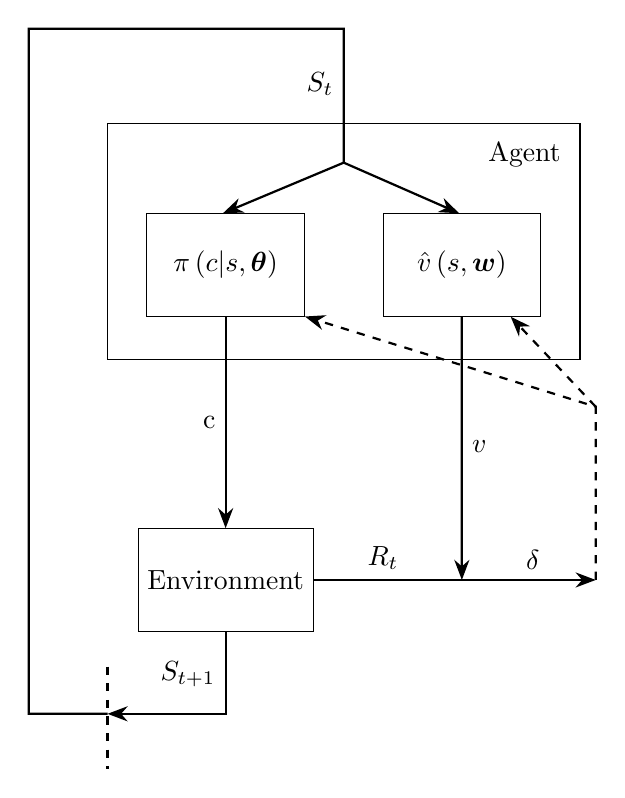
\begin{tikzpicture}[node distance=2cm]
        \node (agent) [process, minimum width=6cm, minimum height=3cm,
            label={[anchor=north east,inner sep=7pt]north east:Agent}]{};
        \node (pi) [process, left of=agent, xshift=0.5cm, yshift=-0.3cm]
            {\(\pi\left(c\middle|s,\bm{\theta}\right)\)};
        \node (v) [process, right of=pi, xshift=1cm]
            {\(\hat{v}\left(s,\bm{w}\right)\)};
        \node (env) [process, below of=pi, yshift=-2cm] {Environment};

        \draw [arrow] (pi) -- node[anchor=east] {c} (env);
        \draw [arrow] (env)
            -- ++(0,-1.7) node[anchor=east, yshift=0.5cm] {\(S_{t+1}\)}
            -- ++(-1.5,0) coordinate(next_s);
        \draw [arrow] (next_s) -- ++(-1,0) -- ++ (0,8.7) -- ++(4,0)
            -- ++(0,-1.7)
            node[anchor=east, yshift=1cm] {\(S_t\)} coordinate(m1)
            -- (pi.93);
        \draw [arrow] (m1) -- (v.93);
        \draw [arrow] (env)
            -- ++(3,0) coordinate(m2) node[anchor=south, xshift=-1cm] {\(R_t\)}
            -- +(1.7,0)
            node[anchor=south, xshift=-0.8cm] {\(\delta\)} coordinate(m3);
        \draw [arrow] (v) -- (m2) node[anchor=west, yshift=1.7cm] {\(v\)};
        \draw [dashed,arrow] (m3) -- ++(0,2.2) coordinate(m4) -- (pi.327);
        \draw [dashed,arrow] (m4) -- (v);
        \draw [dashed, thick] (-3,-5.4) -- (-3,-6.7);
    \end{tikzpicture}
    \caption{Actor-Critic for Finance Algorithm Illustration}
    \label{fig:a2c-illustration}
\end{figure}

\subsection{Training Result}
\noindent Figure~\ref{fig:a2c-out} shows the training result of 
Algorithm~\ref{algorithm:actor-critic} (300 moving average reward vs 
iteration), with 600 iterations (5 episodes per iteration), \(T=300\), 
\(\gamma=0.99\), \(\alpha_\theta=\alpha_{\bm{w}}=\num{3e-4}\).
\begin{figure}
    \centering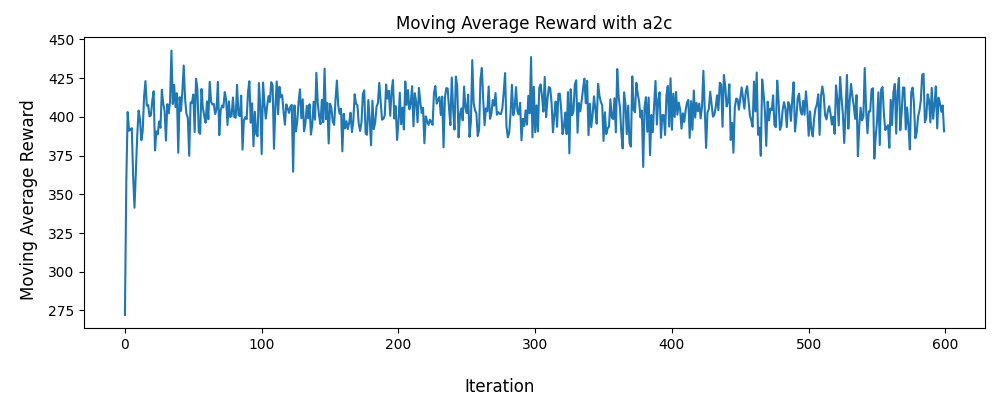
\includegraphics[scale=0.65]{a2c_out}
    \caption{Training Result for Algorithm a2c}
    \label{fig:a2c-out}
\end{figure}
The graph shows that the moving average reward converges within only 50
iterations, that is, 250 episode, 75000 parameter updates for each network,
and stays quite stable afterwards.

\section{Actor-Critic, Reinforce, and PPO}
\subsection{Algorithms}
\noindent To further show how Actor-Critic algorithm performs, we compare it 
to another two popular algorithms: REINFORCE~\cite{williams1992simple}
(Algorithm~\ref{algorithm:reinforce}) and PPO~\cite{schulman2017proximal} 
(Algorithm~\ref{algorithm:ppo}).
The policy function of the two algorithms is implemented the same way as we 
did in Actor-Critic algorithm, and the same is true for the value function 
used in PPO method.
\begin{algorithm}
    \caption{Reinforce for financial problem~\cite{Sutton1998}}
    \label{algorithm:reinforce}
    \begin{algorithmic}[1]
        \State Initialize ANN policy parameterization
        \(\pi\left(c\middle|s, \bm{\theta}\right)\), with any \(\bm{\theta}\)
        \State Step sizes \(\alpha_{\bm{\theta}}>0\)
        \Loop \hspace{0.3mm} (for each episode)
        \State Reset the environment
        \State Generate an episode 
        \(S_0, C_0, R_1, ..., S_{T-1}, C_{T-1}, R_T\),
        following \(\pi\left(\cdot\middle|\cdot, \bm{\theta}\right)\)
        \For{\(t=0, 1, ..., T\)}
        \State \(G \gets \sum_{k=t+1}^{T} \gamma^{k-t-1}R_k\)
        \State \(\bm{\theta} \gets \bm{\theta} + \alpha_{\bm{\theta}}\gamma^t
        G\nabla{\ln{\pi\left(C_t\middle|S_t, \bm{\theta}\right)}}\)
        \EndFor
        \EndLoop
    \end{algorithmic}
\end{algorithm}

\begin{algorithm}
    \caption{PPO for financial problem~\cite{SpinningUp2018}}
    \label{algorithm:ppo}
    \begin{algorithmic}[1]
        \State Initialize ANN policy parameterization
        \(\pi\left(c\middle|s, \bm{\theta}\right)\), with any \(\bm{\theta}\)
        \State Initialize ANN state-value function parameterization
        \(\hat{v}(s,\bm{w})\) with any \(\bm{w}\).
        \State Step sizes \(\alpha_{\bm{\theta}}>0\), \(\alpha_{\bm{w}}>0\)
        \For{iteration \(k=0, 1, 2, ...\)}
        \State Collect set of trajectories \(\mathcal{D}_k=\{\tau_i\}\),
        following \(\pi\left(\cdot\middle|\cdot, \bm{\theta}_k\right)\), where
        \(\tau = S_0, C_0, R_1, ..., S_{T-1}, C_{T-1}, R_T\)
        \For{\(t=0, 1, ..., T\) in each trajectory \(\tau\) in 
        \(\mathcal{D}_k\)}
        \State \(G_t \gets \sum_{k=t+1}^{T} \gamma^{k-t-1}R_k\)
        \State \(A_t \gets G_t - \hat{v}(S_t)\)
        \EndFor
        \Loop \hspace{0.3mm} (update multiple times)\vspace{1mm}
        \State \(\bm{\theta} \gets \underset{\bm{\theta}}{\text{arg\:max}}
        \frac{1}{|\mathcal{D}_k|T}
        \sum_{\tau\in\mathcal{D}_k}^{} \sum_{t=0}^{T}
        \min{\left(
                \frac{\pi\left(c_t\middle|S_t, \bm{\theta}\right)}
                {\pi\left(c_t\middle|S_t, \bm{\theta}_k\right)}A_t,
                \text{clip}\left(
                    \frac{\pi\left(c_t\middle|S_t, \bm{\theta}\right)}
                    {\pi\left(c_t\middle|S_t, \bm{\theta}_k\right)},
                    1-\epsilon, 1+\epsilon
                \right)A_t
        \right)}\)
        \State \(\bm{w} \gets \underset{\bm{w}}{\text{arg\:min}}
        \frac{1}{|\mathcal{D}_k|T}\sum_{\tau\in\mathcal{D}_k}^{} \sum_{t=0}^{T}
        \Bigl(\hat{v}(S_t, \bm{w})-G_t\Bigr)^2\)
        \EndLoop
        \EndFor
    \end{algorithmic}
\end{algorithm}

\subsection{Training result}
\noindent Figure~\ref{fig:3-algorithms-out} shows the training 
result of these three algorithms (300 moving average reward vs iteration), 
with 600 iterations (5 episodes per iteration), \(T=300\), \(\gamma=0.99\),
\(\alpha_\theta=\num{3e-4}\), \(\alpha_{\bm{w}}=\num{3e-10}\) (if applicable),
\(\epsilon=0.5\) (if applicable).
\begin{figure}
    \centering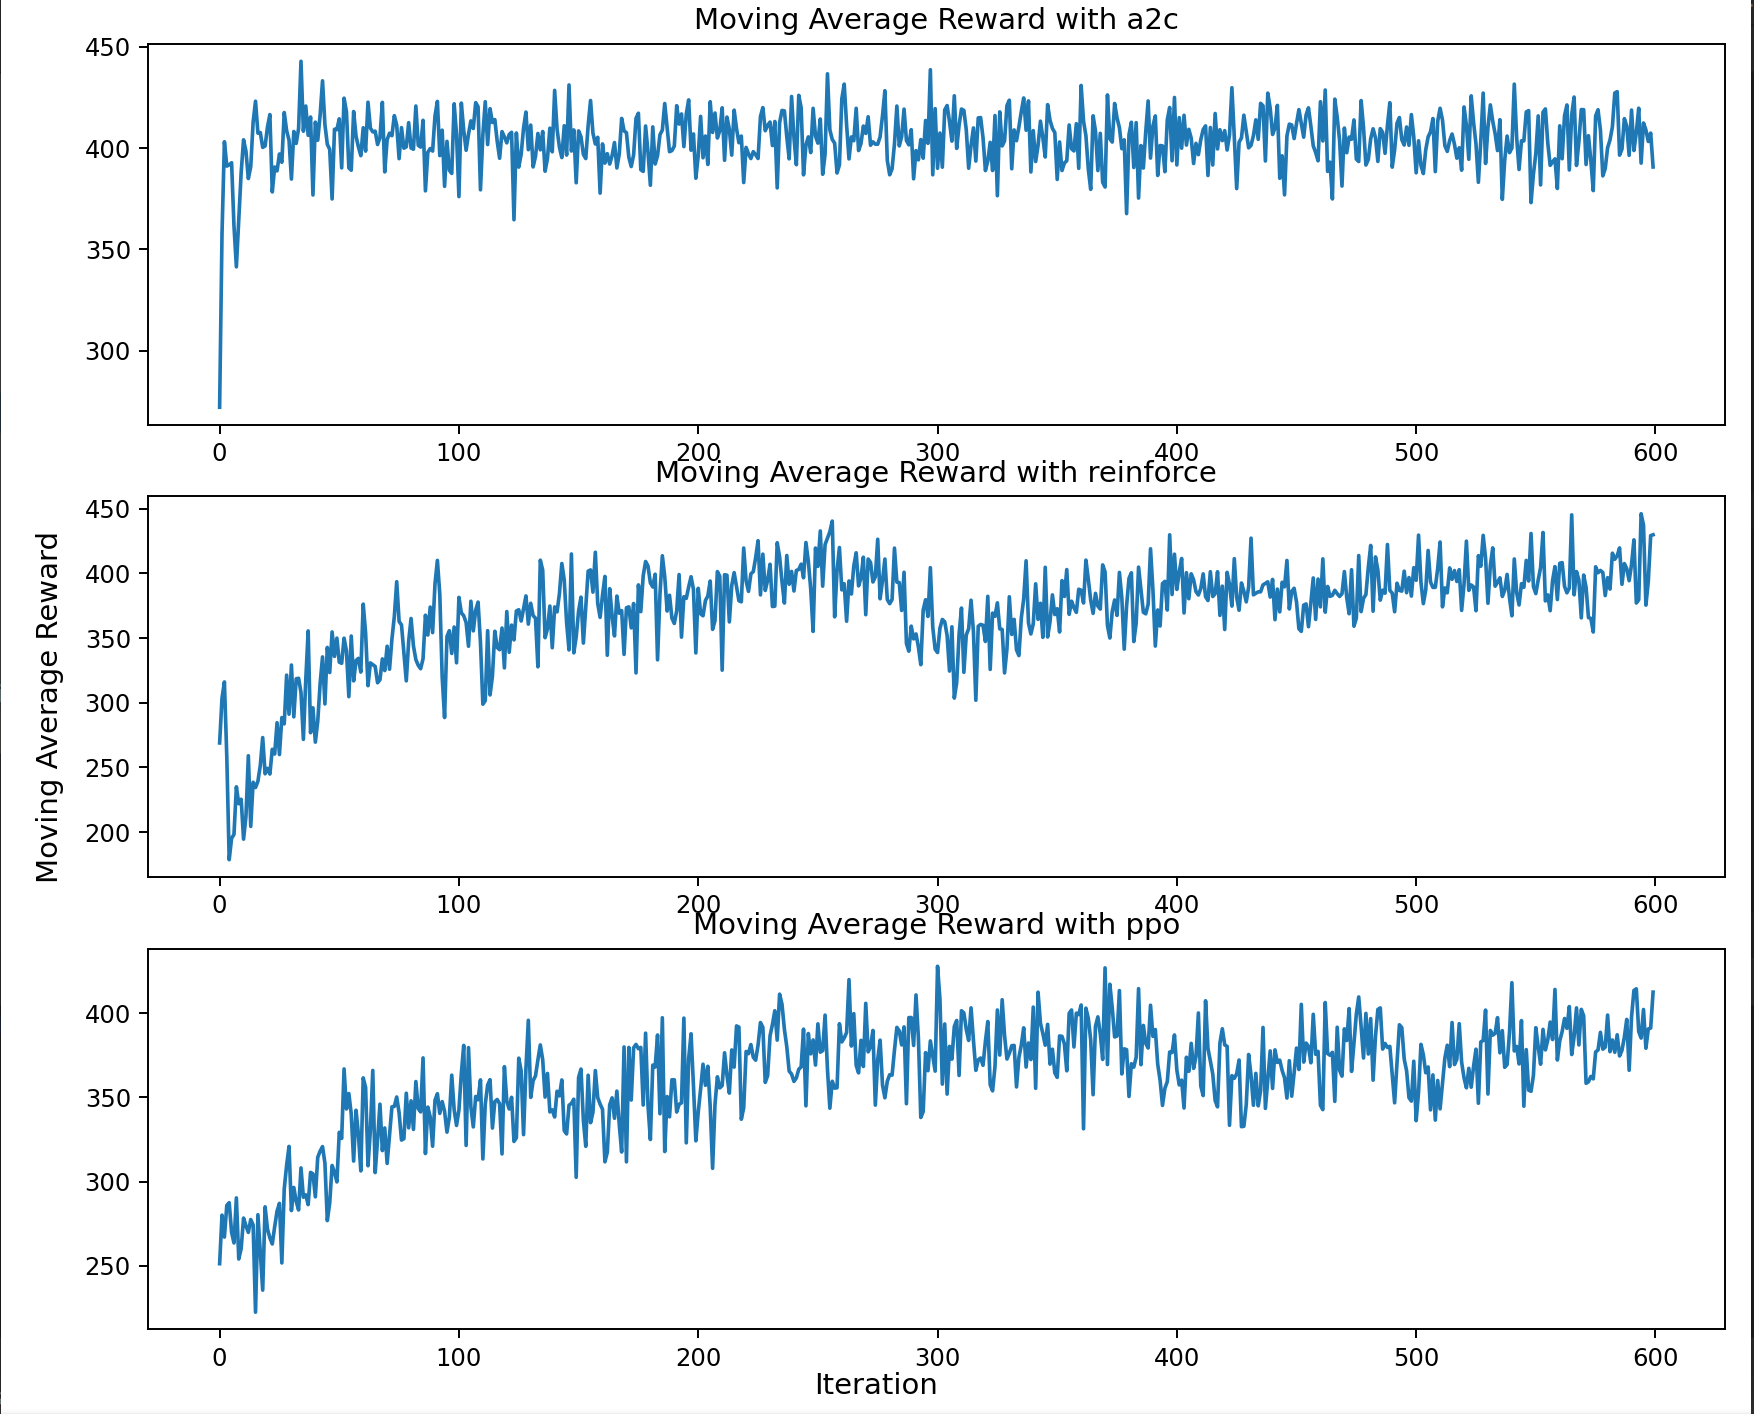
\includegraphics[scale=0.65]{out}
    \caption{Training Result Comparison for Three Algorithm}
    \label{fig:3-algorithms-out}
\end{figure}
As we can see, the Actor-Critic algorithm converges the fastest, within 50 
iterations, followed by REINFORCE algorithm, which converges within 250 
iterations, despite a small drop of moving average around iteration 300, 
which is quickly corrected by the algorithm within 50 iterations. PPO 
algorithm converges the slowest, with about 300 iterations.

\section{Conclusion}
\noindent To summarize, the moving average rewards after convergence of these 
three algorithms are nearly the same (around 400), which is as expected. 
The Actor-Critic algorithm performs really well compared to anther two 
algorithms, it has highest converge rate, the reward is also very stable after 
convergence. 
In the mean time, the slow convergence for PPO algorithm is expected since it 
uses a clip function to prevent model from changing too fast in a single 
update~\cite{schulman2017proximal, SpinningUp2018}, although at current stage 
it seems to be unnecessary for our specific problem setup. 
Further investigation needs to be done for the unexpected small drop of the 
reward for the REINFORCE algorithm.

\bibliographystyle{unsrt}
\bibliography{references}

\end{document}

